\section{Charaterization}
    %%%%%%%%%%%%%%%%%%%%%%%%%%%%%%%%%%%%%
	%%  Slide 1: <> %%
	%%%%%%%%%%%%%%%%%%%%%%%%%%%%%%%%%%%%%
    \begin{frame}
        \frametitle{Threshold and noise}
        The threshold and the noise are \textbf{strictly} related with the \textbf{FE} status, and in particular to the threshold of the \textbf{discriminator}.\\
        \medskip
        The lower the threshold, the lower the minium detectable signal, allowing for thinner detector (Q$_{MIP}\sim$\SI{80}{e/\um}). \\
        \medskip
        What determins the minimum stable threshold?
        \begin{itemize}
            \item the \textbf{ENC} 
            \item the \textbf{threshold dispersion} 
            \item threshold variation in \textbf{time}
        \end{itemize}
        \medskip
        \centering\begin{beamercolorbox}[sep=0em,wd=0.85\textwidth,ht=1.5ex, dp=0.1ex, rounded=true, center]{lightbluebox}
            noise \SI{9}{\elementarycharge}$^-$    threshold \SI{270}{\elementarycharge}$^-$    threshold dispersion\SI{30}{\elementarycharge}$^-$
        \end{beamercolorbox}
    \end{frame}


    %%%%%%%%%%%%%%%%%%%%%%%%%%%%%%%%%%%%%
	%%  Slide 1: <Scurve> %%
	%%%%%%%%%%%%%%%%%%%%%%%%%%%%%%%%%%%%%
    \begin{frame}
        \frametitle{Threshold and noise: how measure them?}
        \textbf{Injection circuit}: allows injecting a fixed charge Q on a capacity (C$_{inj}$=\SI{230}{fF}) at the FE input
        \bigskip
        \begin{columns}
            \column{0.45\textwidth}           
                  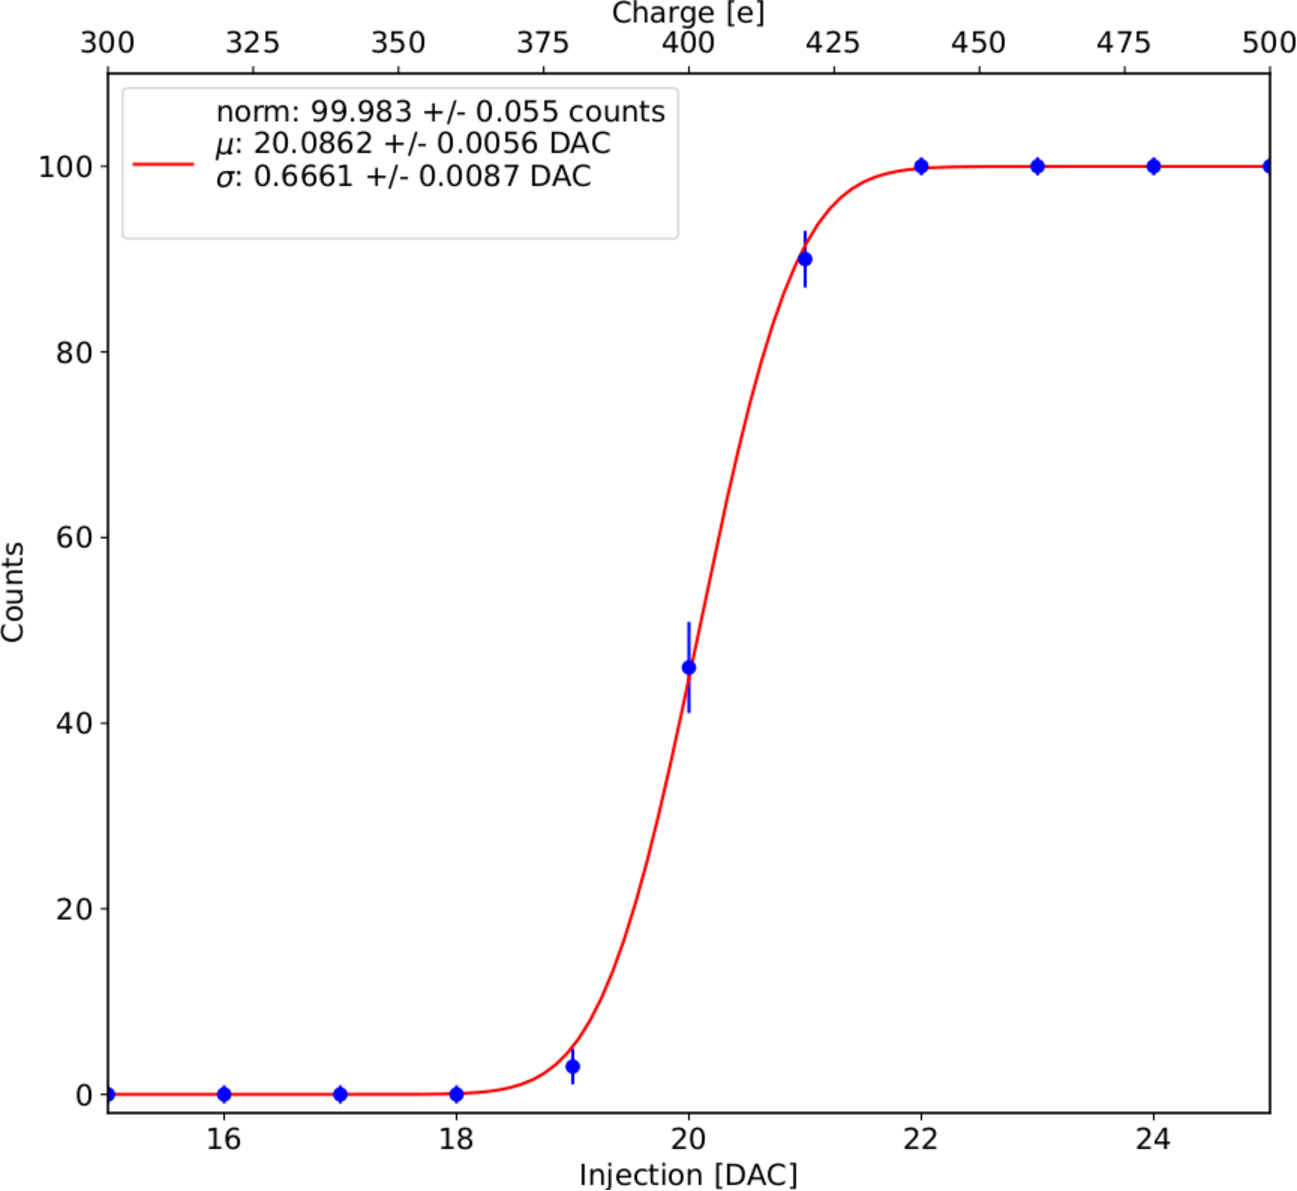
\includegraphics[width=1.1\linewidth]{figures/charaterization/scurve.pdf}
            \column{0.55\textwidth} 
                %\begin{center}
                \begin{beamercolorbox}[sep=0em,wd=0.45\textwidth,ht=1.5ex, dp=0.1ex, rounded=true, center]{lightbluebox}
                    F=\SI{20}{\elementarycharge}$^-$/DAC
                \end{beamercolorbox}
                %\end{center}                    
                \\
                \bigskip
                Assuming a gaussian noise:
                \begin{itemize}
                    \item the threshold is the 50\%
                    \item the noise is 1/slope 
                \end{itemize}
                \medskip
                Analitical parametrization of the curve with $error\,function$
                %\begin{equation*}
                %    \tiny
                %    f(x, \mu, \sigma) = \frac{1}{2} \; \left(1\,+\,erf\left(\frac{x-\mu}{\sigma \sqrt{2}}\right)\right)
                %    \label{eq:fit_scurve}
                %\end{equation*}
        \end{columns}
    \end{frame}


    %%%%%%%%%%%%%%%%%%%%%%%%%%%%%%%%%%%%%%%%
    %%  Slide 2: <Threshold_noise>  %%
    %%%%%%%%%%%%%%%%%%%%%%%%%%%%%%%%%%%%%%%%
    \begin{frame}
        \frametitle{Threshold and noise}

            \begin{figure}
                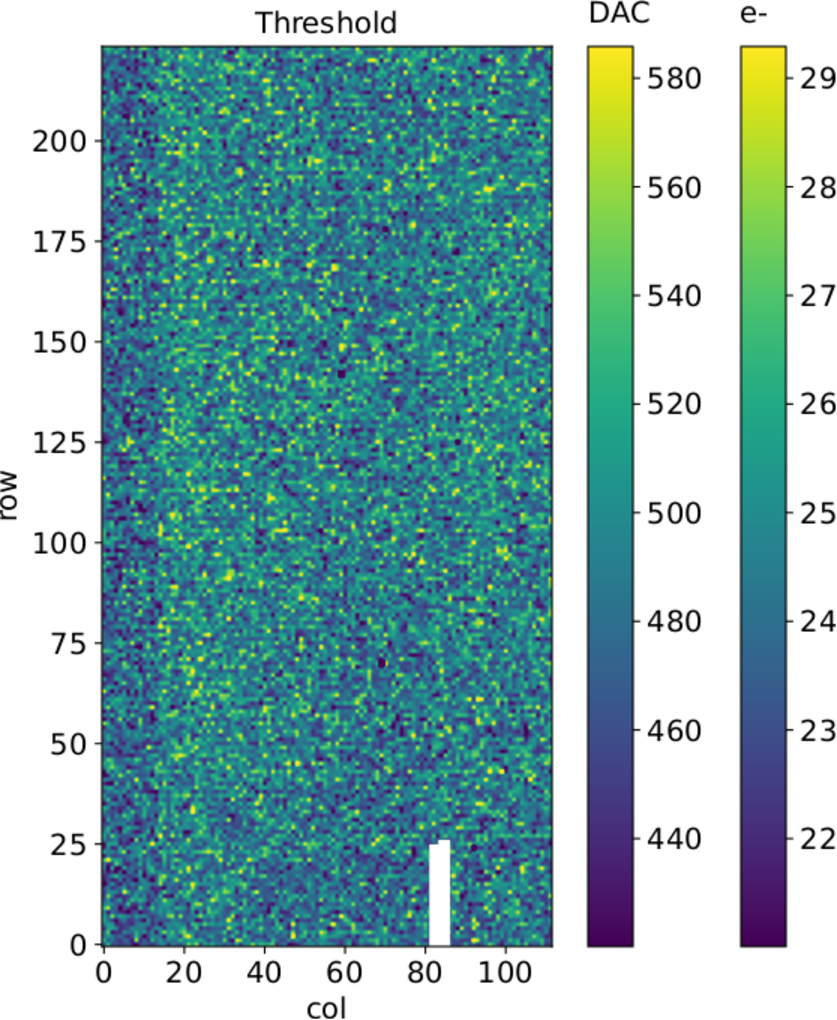
\includegraphics[width=.45\linewidth]{figures/charaterization/threshold_map.pdf}
                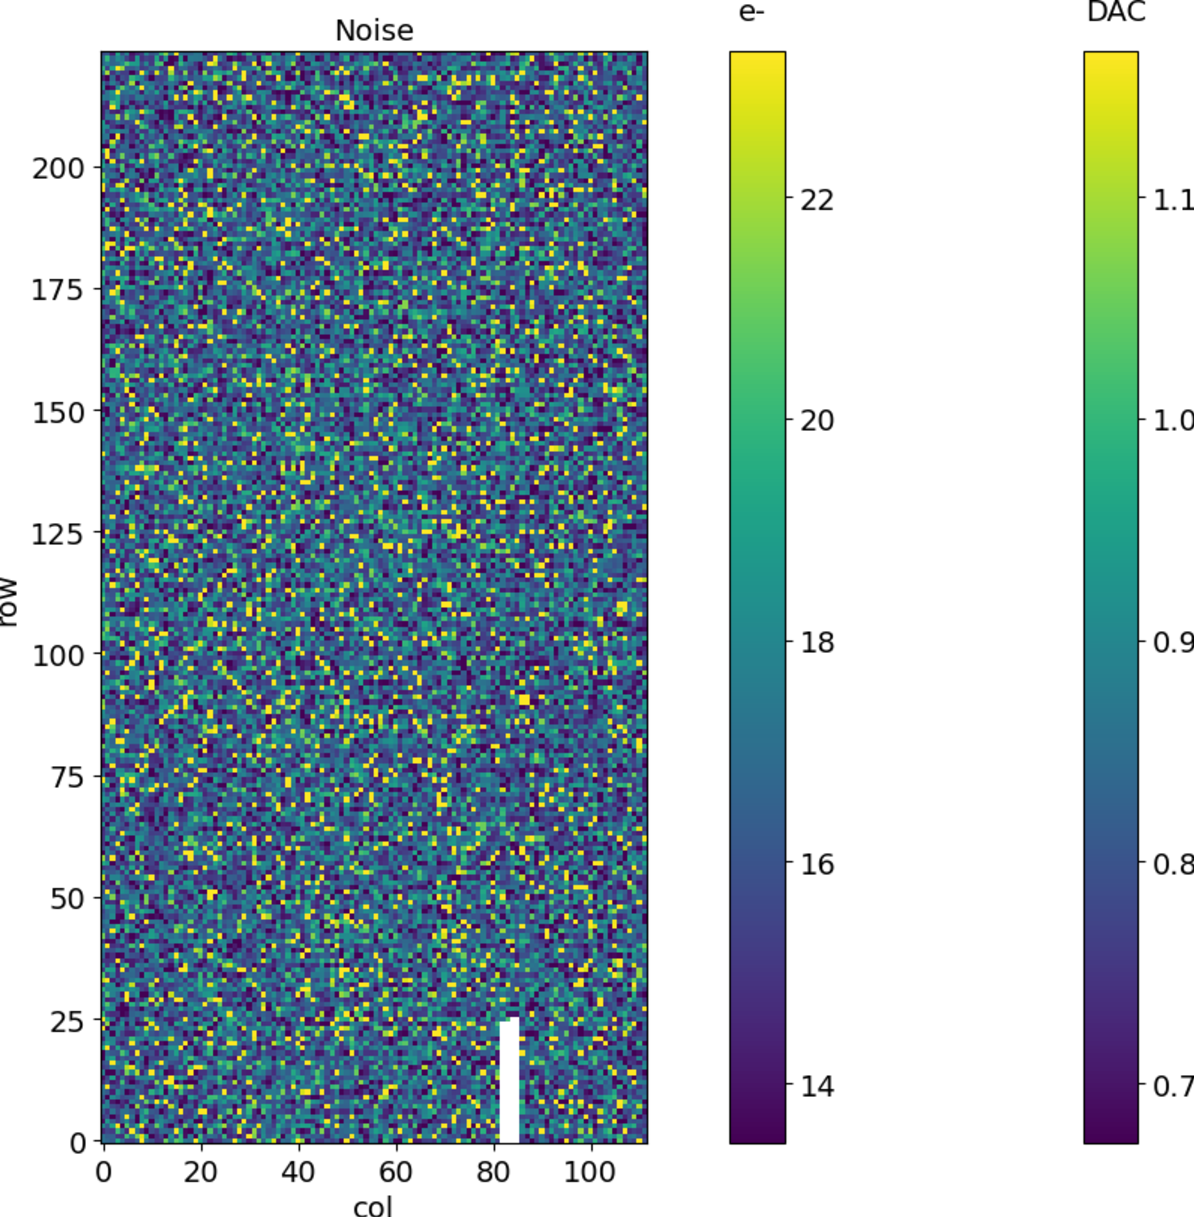
\includegraphics[width=.45\linewidth]{figures/charaterization/noise_map.pdf}                
            \end{figure}

        Injection circuit broken.\\
        With this threshold the mean rate is $\sim$\SI{3}{Hz} on all the matrix, excluding the noisy pixels!
        Changing the register which sets the discriminator threshold the effective threshold changes in range (370-500). NEed for more bits and for a fine tuning per pixel
    \end{frame}

    %%%%%%%%%%%%%%%%%%%%%%%%%%%%%%%%%%%%%%%%
    %%  Slide 4: <ToT vs charge>  %%
    %%%%%%%%%%%%%%%%%%%%%%%%%%%%%%%%%%%%%%%%
    \begin{frame}
        \frametitle{Calibration}
        Q injected in DAC depends on the C$_{inj}$, different for each pixel.     
        \bigskip
        How convert the DAC units in electrons collected in the sensor?\\
        \begin{itemize}
            \item take advantage linearity of the output signal 
            \item need of a reference, radioactive source
        \end{itemize}
        \medskip
        \begin{beamercolorbox}[sep=0em,wd=0.85\textwidth,ht=1.5ex, dp=0.1ex, rounded=true, center]{lightbluebox}
            Fe$^{55}$ $\rightarrow$ Mn$^{55}$ + K$_\alpha$ (\SI{5.9}{keV}) or K$_\beta$ (\SI{6.5}{keV})
        \end{beamercolorbox}
        \begin{tikzpicture}[overlay]
            \draw[decorate,decoration={brace}]
                (3.5,0) -- (5.5,0);
        \end{tikzpicture}
        \begin{columns}
            \column{0.2\textwidth}             
            \column{0.8\textwidth}             
            \begin{itemize}
                \item $\lambda$=\SI{29}{\um}$\rightarrow$ P$_{abs}$=
                \item $w_i$=\SI{3.6}{eV} in Si @ \SI{300}{\kelvin}$\rightarrow$ \SI{1616}{\elementarycharge}$^-$
            \end{itemize}
        \end{columns}
    \end{frame}  


    %%%%%%%%%%%%%%%%%%%%%%%%%%%%%%%%%%%%%%%%
    %%  Slide 3: <ToT linearity>  %%
    %%%%%%%%%%%%%%%%%%%%%%%%%%%%%%%%%%%%%%%%
    \begin{frame}
        \frametitle{ToT linearity}
        \begin{itemize}
            \item linearity is due to the \textbf{PMOS} reset circuit of the amplifier which guaranties that the discharge of the preamplifier is costant in time. Then the ToT is completely correlated with the pulse amplitude 
            \item ToT is saved as a 6-bits variable and can ToT varies in range 0-63
        \end{itemize}
        \medskip
        \medskip
        \medskip
        \begin{columns}
            \column{0.6\textwidth}  
                \centering
                Linearity tested with the injection
                \begin{figure}[h!]
                    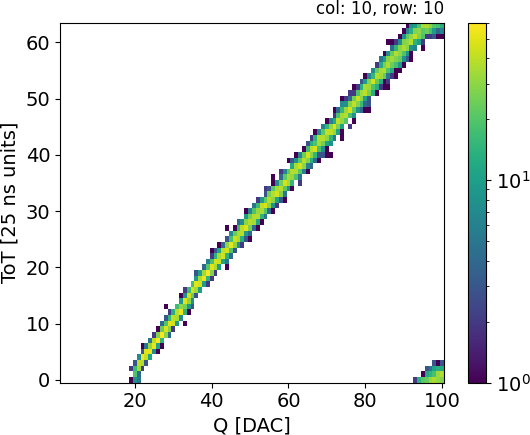
\includegraphics[width=.49\linewidth]{figures/charaterization/ToT_rollover.png}
                    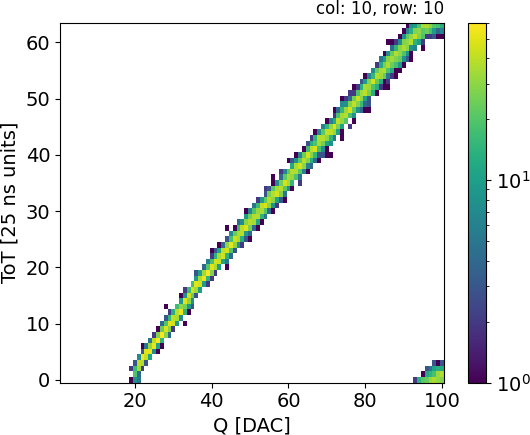
\includegraphics[width=.49\linewidth]{figures/charaterization/ToT_rollover.png} 
                \end{figure}
            \column{0.4\textwidth}
                \centering\textbf{Rollover!}\\
                \smallskip
                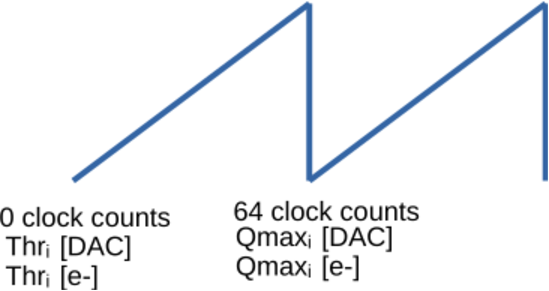
\includegraphics[width=.99\linewidth]{figures/Monopix1/rollover.pdf} 
        \end{columns}
    \end{frame}    
      

    %%%%%%%%%%%%%%%%%%%%%%%%%%%%%%%%%%%%%%%%
    %%  Slide 4: <ToT calibration>  %%
    %%%%%%%%%%%%%%%%%%%%%%%%%%%%%%%%%%%%%%%%
    \begin{frame}
        \frametitle{ToT absolute calibration}
        \begin{columns}
            \column{0.4\textwidth}                  
                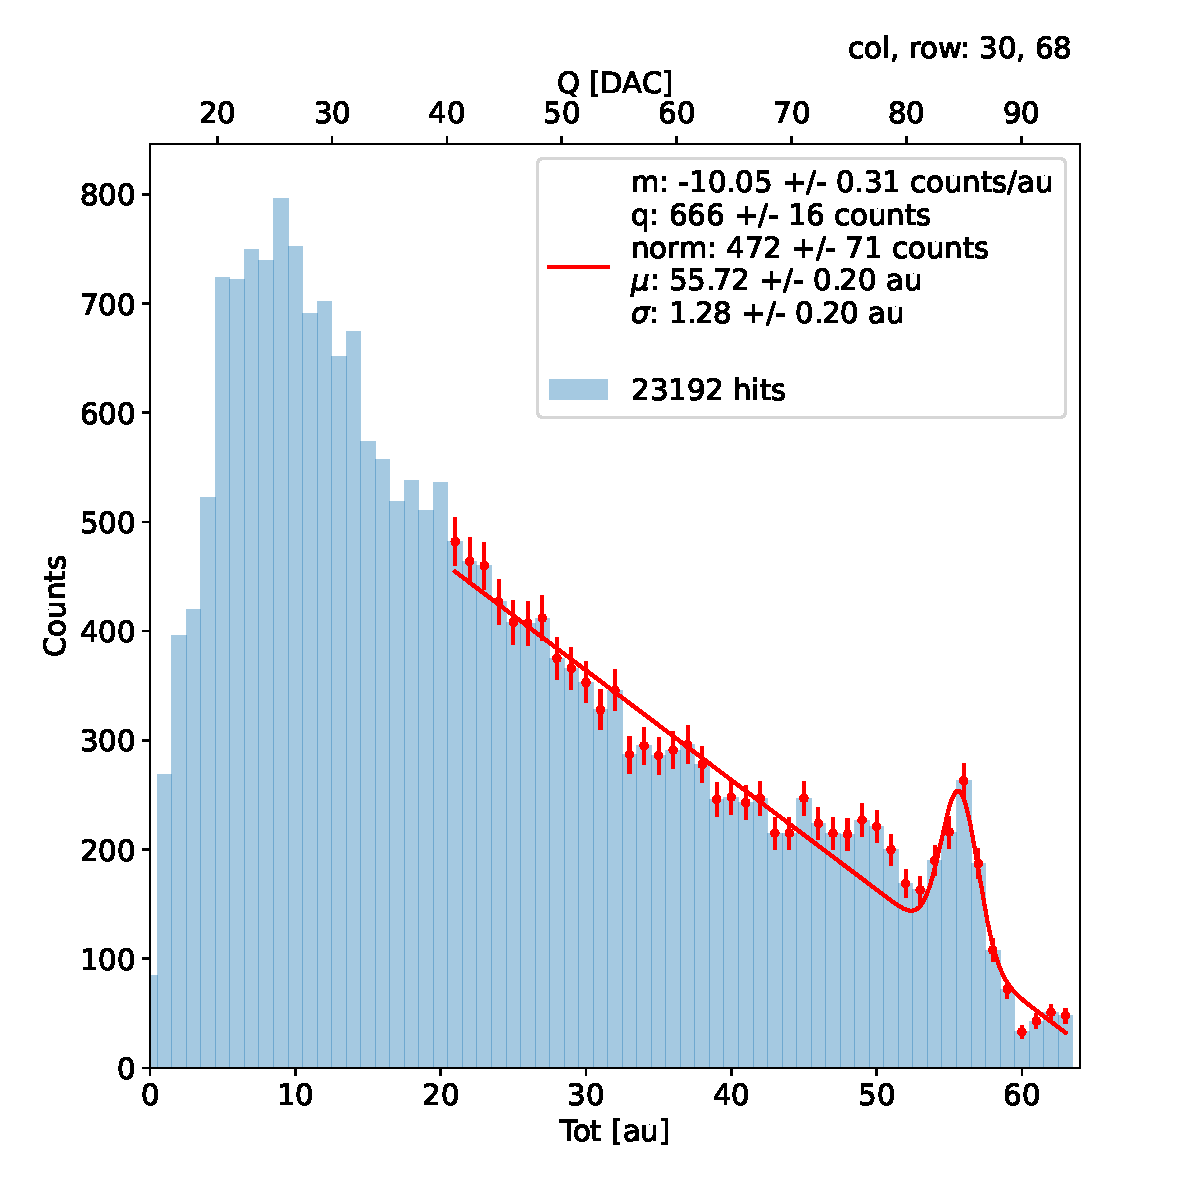
\includegraphics[width=1.1\linewidth]{figures/charaterization/fit_line_gauss_r69.pdf}
            \column{0.4\textwidth}    
            \begin{itemize}
                \item fit to find the peak position in the spectrum
                \item conversion from ToT in DAC (using the line parameters)
                \item peak value in DAC fixed to be equal to \SI{1616}{\elementarycharge}$^-$
            \end{itemize} 
        \end{columns}
        
    \end{frame}     




    %%%%%%%%%%%%%%%%%%%%%%%%%%%%%%%%%%%%%%%%
    %%  Slide 4: <Aquisitions with sources>  %%
    %%%%%%%%%%%%%%%%%%%%%%%%%%%%%%%%%%%%%%%%
    \begin{frame}
        \frametitle{Acquisition with sources}
        \begin{columns}
            \column{0.4\textwidth}                  
                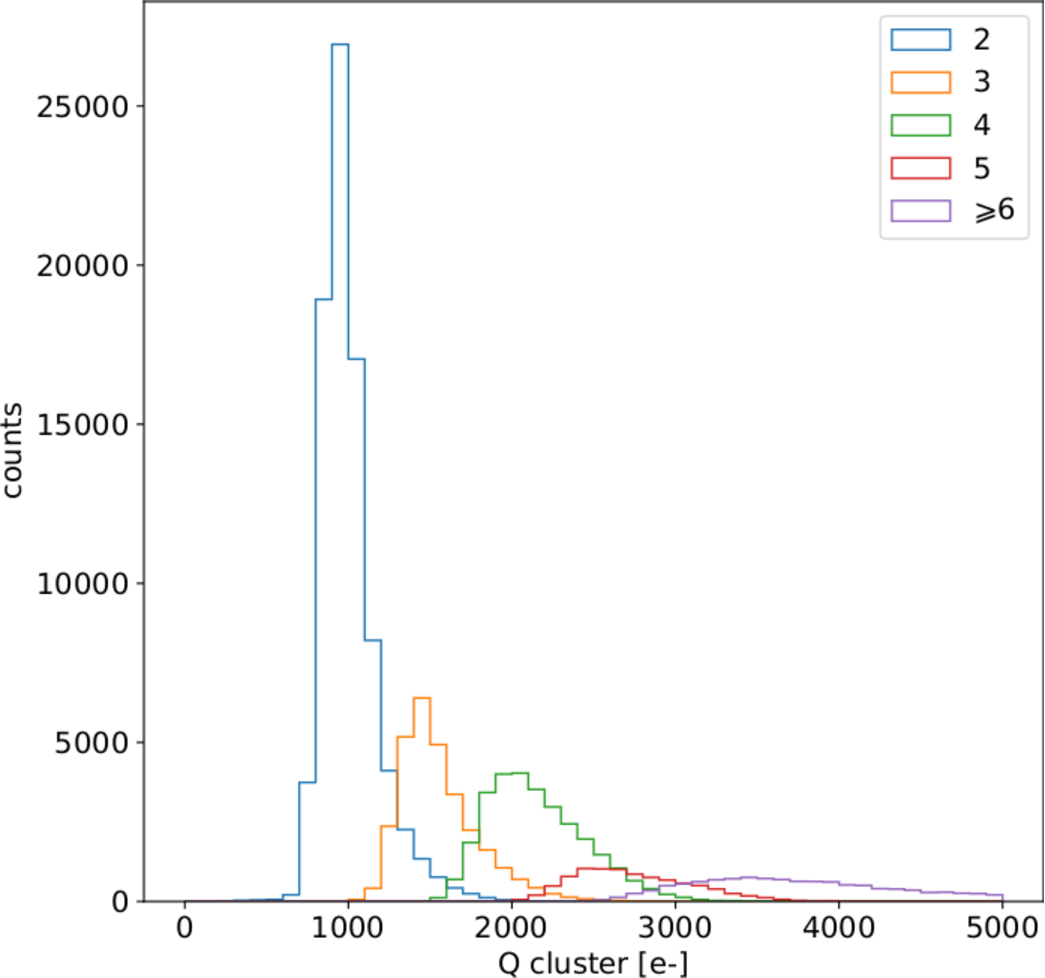
\includegraphics[width=.99\linewidth]{figures/charaterization/Sr90_spectrum_cluster.pdf}
            \column{0.4\textwidth}                  
        \end{columns}
        
    \end{frame}    


    %%%%%%%%%%%%%%%%%%%%%%%%%%%%%%%%%%%%%%%%
    %%  Slide 5: <ToT bias>  %%
    %%%%%%%%%%%%%%%%%%%%%%%%%%%%%%%%%%%%%%%%
    \begin{frame}
        \frametitle{Changing the bias}
        \begin{columns}
            \column{0.3\textwidth} 
                Acquisitions with:
                \begin{itemize}
                    \item Injection
                    \item Fe$^{55}$ source
                \end{itemize}
            \column{0.7\textwidth} 
                %Maximum bias suggested
                \begin{table}
                    \begin{center}
                    \scalebox{0.75}{
                    \begin{tabular}{| c |  c | c | c |}
                    \hline
                    & -\SI{6}{V} & -\SI{3}{V} & \SI{0}{V}\\
                    \hline
                    \hline
                    Threshold [DAC] & 20 $\pm$ 2 & 21 $\pm$ 2 & 24 $\pm$ 2\\
                    Noise [DAC] & 0.61 $\pm$ 0.08 & 0.62 $\pm$ 0.08 & 0.82 $\pm$ 0.1\\
                    \hline
                    \end{tabular}}
                    \end{center}
                \end{table}
        \end{columns}
 
        \begin{columns}
            \column{0.4\textwidth}          
            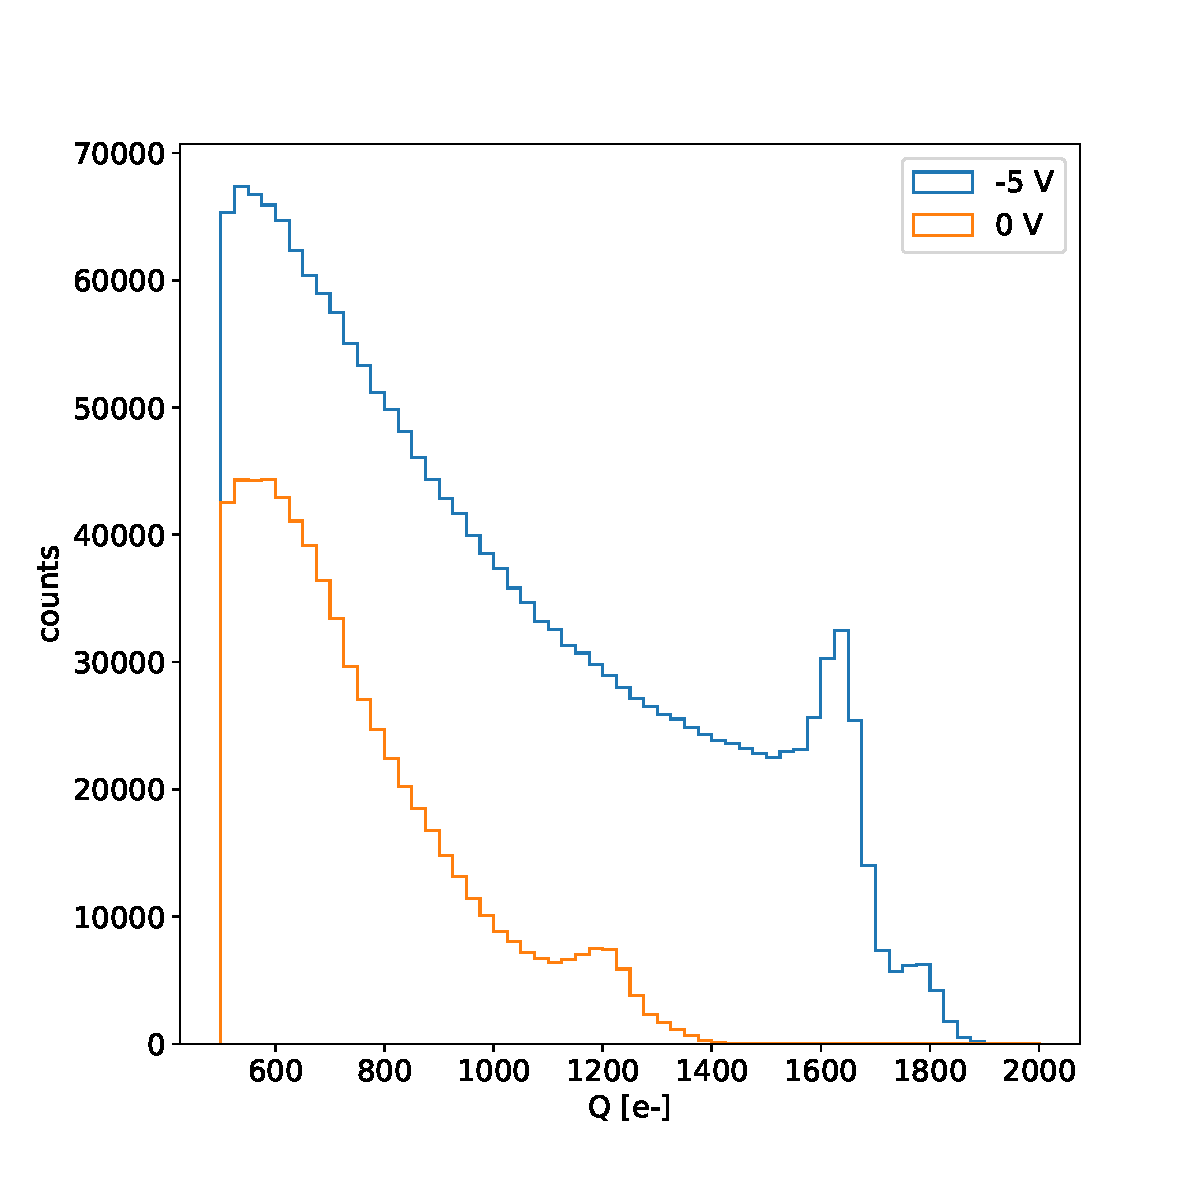
\includegraphics[width=1.2\linewidth]{figures/charaterization/Fe_spectrum_bias.pdf}
        \column{0.6\textwidth}
            Reducing the bias from -\SI{6}{V} to \SI{0}{V} eduction of the below quantity in the Fe$^{55}$ spectrum: 
            \begin{itemize}
                \item ToT value of the peak $\sim$30\%
                \item N of events under the peak $\sim$60\%
                \item hit rate $\sim$60\%
            \end{itemize}
          
        \end{columns}
    \end{frame}      

    %%%%%%%%%%%%%%%%%%%%%%%%%%%%%%%%%%%%%%%%
    %%  Slide 5: <Dead time>  %%
    %%%%%%%%%%%%%%%%%%%%%%%%%%%%%%%%%%%%%%%%
    \begin{frame}
        \frametitle{Readout time}
        \textbf{Injection} allows injecting pulses at different rate. 
        \begin{itemize}
            \item no memory on pixel: 
            \item readout is completely sequential: one serializer @ \SI{40}{MHz}
            \item each hit is a 27-bits data packet, at least \SI{675}{ns} needed
        \end{itemize}

        \medskip
        \begin{columns}
            \column{0.55\textwidth}              
                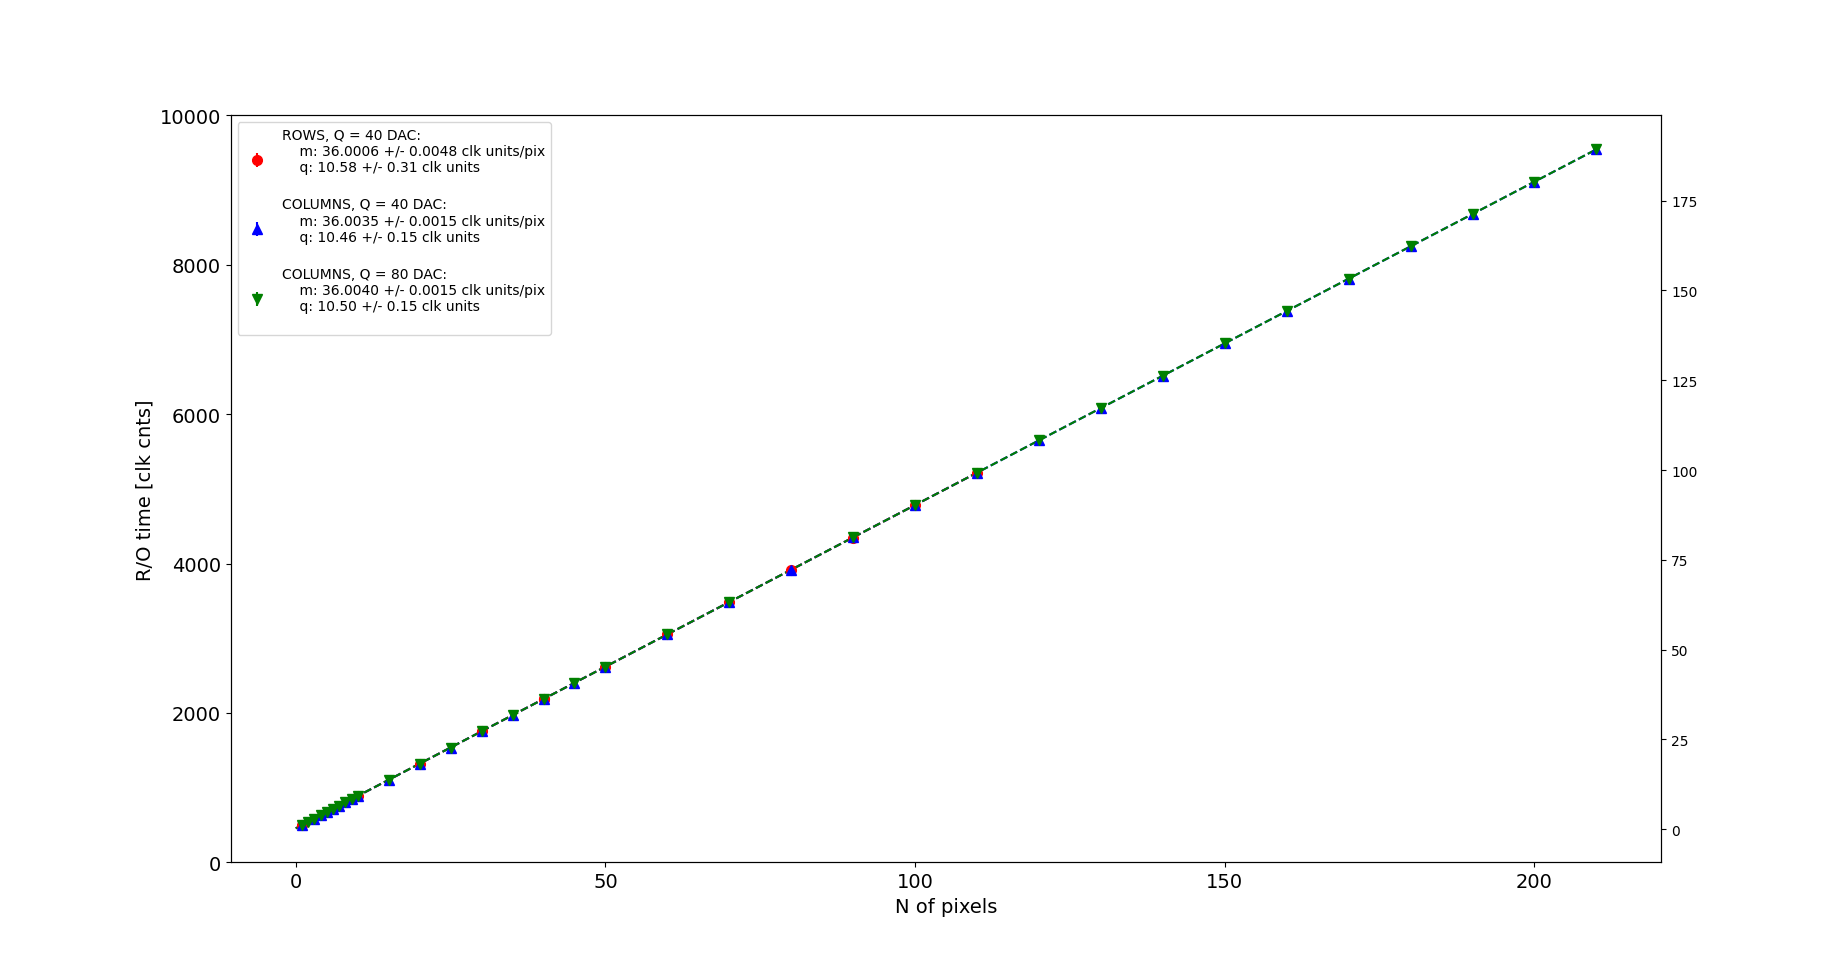
\includegraphics[width=1.07\linewidth]{figures/charaterization/default_line.pdf}
            \column{0.45\textwidth}  
            Readout time \textbf{slightly} depends on the FE status and can be reduced down to \SI{31}{clk.}cnts = \SI{775}{ns} per pixels 

        \end{columns}            
    \end{frame}          